\section{Literature review}
This section will briefly outline the main state-of-the-art models related to this project.

At the moment, research is mainly focused on recognizing named entities within clinical texts; for example, these are: symptoms, tests, treatments, medications and chemical names. Hence, as shown in table \ref{tab:comparativeNER}, the available models are not specialized in classifying symptoms: they simply perform \textit{Named Entity Recognition} (NER).

An experimental comparison of different Machine-Learning approaches to medical entity recognition is presented in \cite{liu2017}. This work investigate the performance of LSTM (long-short term memory), a representative variant of RNN, on clinical entity recognition. It concludes that LSTMs perform only slightly better than Structured Support Vector Machines (SVM) on this task.

In addition, the publicly available recognition systems of symptoms are rare. This because of the diversity and complexity of symptom named entities in naming conventions and the lack of appropriate training corpora \cite{wei2016disease}. In order to avoid the first problem, this work proposes to map the symptoms identified in text to a medical standard classification (MEDCIN).
 
However, while symptom identification (i.e. recognition) has been recently investigated, symptom classification has not yet been studied. Nevertheless, as discussed in section \ref{sub:whyclassifying}, mapping symptoms towards a standard classification can be useful for eventual future components based on this work.

\hspace*{2in}
\begin{table}[h]
  \centering
  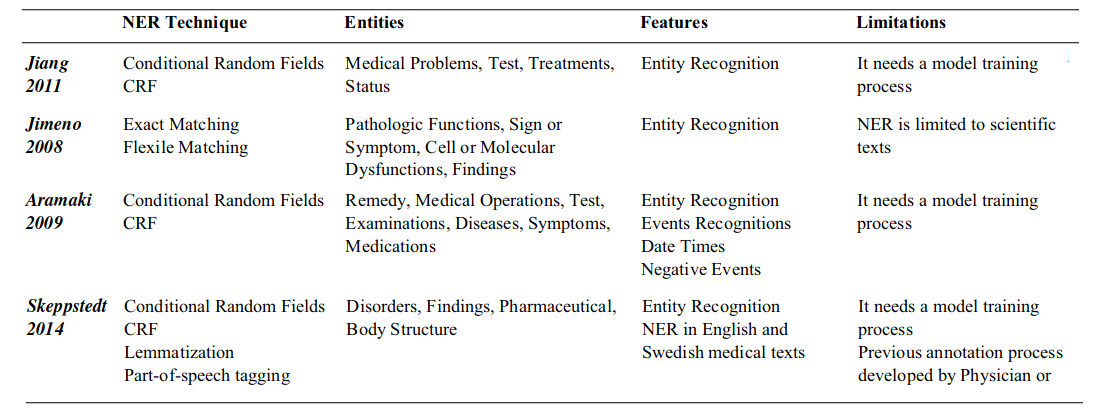
\includegraphics[width=17.5cm]{comparisonNER}
  \caption{Comparative analysis of various methods of NER in medical texts (Jiang et al. \cite{jiang2011}, Jimeno et al. \cite{jimeno2008}, Aramaki et al. \cite{aramaki2009} and Skeppstedt et al. \cite{skeppstedt2014}). Table taken from \cite{NERoverEHR}.}
  \label{tab:comparativeNER}
\end{table}
